\chapter{Requirements and tools}
\label{chap:req-and-tools}

The project development consisted of multiple stages. One of the most important parts was specifying requirements, which then dictated tool selection and the design process.

\section{Functional requirements}

Functional requirements list functionality available in the system. Each of the requirements contains a description detailing the desired behaviour.

\begin{enumerate}
	\item \textbf{Account creation}: Users must be able to register an account in the system.
	This operation requires username and password submission from an HTML form in a POST request.
	Registration is allowed only using unique username. If there already exists an account in the system with the same username, the action must be refused.
	As a result of a successful registration, a document with the username, cryptographic hash of the user's password and a default role \texttt{"user"} is inserted into a collection storing user accounts. After the registration succeeds, the user is redirected to the login page.

	\item \textbf{Signing in}: Users must be able to log into their accounts.
	Username and password must be sent in a POST request as HTML form data. The operation must fail if there is no account in the database with the provided username or if the password hash does not match the one stored in the database.
	If there has been no failure, a session is created and the user is redirected to the home page.

	\item \textbf{Logging out}: Users must be able to log out of their accounts.
	It is expected that the user is signed in when they log out. This operation destroys the session (if any) and redirects to the home page.

	\item \textbf{Changing password}: Users must be able to change their account password.
	New password must be sent in a POST request as HTML form data. User must be logged in in order to change the password.
	As a result of this operation, user's password hash in the database is updated.

	\item \textbf{Listing categories}: Users must be able to see a list of categories that exist in the system. List of categories must link to category pages.

	\item \textbf{Displaying category}: Users must be able to see category details on a category page. The details should include category name, description and a list of related tasks.

	\item \textbf{Displaying task}: Users must be able to display task details on task pages. The details should include task name, description, challenge URL, hints (if any), and if the user is logged in, a flag submission form. If the task has been solved by the user, instead of the flag submission form, a question is displayed.

	\item \textbf{Solving challenge}: Users must be able to submit a form with flag from the task page. This action is allowed only for signed in users. Submitted flag must be verified with the one stored in the database for the given challenge. If the flags match, a success message should be shown to the user and date of solving the challenge by user ought to be saved to the database. Otherwise, a message informing the user about incorrect flag should be presented.

	\item \textbf{Answering quiz}: User who have solved the main challenge from a task, should be able to see a question on the task page and be able to answer it. Only signed in users can submit answers. Checkboxes which status indicates whether the user thinks that they are correct must be presented along answers from the database. After the answers are submitted, the quiz should be disabled without a button to submit, checkboxes disabled and reflecting the user's answer and an indication which answers were correct.

	\item \textbf{Administrator panel}: Users with the \texttt{"admin"} role (administrators) should have access to a separate administration panel. The panel should expose additional functionality related to the system management.

	\item \textbf{Listing users}: Users with access to the administrator panel should be able to get a list of user account in the system. Each entry must contain information about username and user role. The list should be paginated as there may exist many accounts.

	\item \textbf{Changing user permissions}: Administrators should be able to grant the \texttt{"admin"} role to other users, as well as change it back to \texttt{"user"}.

	\item \textbf{Deleting user}: Administrators should be able to remove user accounts from the database. It must not be possible to remove own user account this way.

	\item \textbf{Creating category}: Administrators must be able to create new categories. The categories must have a name and description. The description must support Markdown input.

	\item \textbf{Editing category}: Administrators must be able to edit the name and description of existing categories.

	\item \textbf{Creating task}: Administrators must be able to add new tasks to the system. For each task it must be possible to set the name, description (in Markdown), hints, challenge details, question, answers to the question. Each answer must be marked as correct or incorrect.\\
	Challenge details must include:
	\begin{itemize}
		\item Docker image to pull and start,
		\item subdomain used for serving the challenge,
		\item flag that the users will try to find,
		\item an interval specifying how frequently the challenge container should be regenerated
	\end{itemize}

	\item \textbf{Starting challenges}: The system must be able to pull challenge images, create and containers and direct connections to specified subdomains into appropriate containers. This must be done automatically during system startup and for each new challenge added when creating new tasks.
\end{enumerate}

\section{Non-functional requirements}

\begin{enumerate}
	\item \textbf{Responsiveness}: UI should properly scale across different display sizes. It must be mobile-friendly.

	\item \textbf{Accessibility}: There should be no errors in the Accessibility section of a \href{https://webhint.io/}{webhint} scan.

	\item \textbf{Visual consistency}: A single set of styling rules, such as colours, fonts and icons should be used across whole user interface.

	\item \textbf{Page load performance}: The system should have a score of over 90 in \href{https://pagespeed.web.dev}{PageSpeed Insights} report for mobile.

	\item \textbf{Compatibility}: User interface should work in latest (as of January 2023) versions of Firefox, Firefox ESR, Chrome and Safari browsers for desktops and mobile devices. Basic system functionality, except for the administrator panel, should be available in browsers with JavaScript disabled.
\end{enumerate}

\section{Use cases}

The use case diagram presented on Fig. \ref{fig:use-case-diag} shows actions offered to actors using the system. There are two actors, with different sets of allowed interactions. The actor \textit{User} represents anyone with access to the system. Users with special account role \texttt{"admin"}, which allows them to perform operations related to management of the system.

\begin{figure}
	\centering
	\includesvg[scale=0.9]{uml/render/usecase.svg}
	\caption{Use case diagram}
	\label{fig:use-case-diag}
\end{figure}

\section{Tools}

The implementation of the project significantly benefited from publicly available tools. Used tools are divided into two classes, depending on the way they were used.

\subsection{Core tools}

The system is built on tools, which are regarded to as \textit{core tools}. These are required for operation and are a part of the system architecture.

\subsubsection{Node.js + Express + EJS}

Node.js is a JavaScript runtime based on V8 engine. There is an enormous ecosystem built around Node.js with over 1.3 million packages available in the npm registry \cite{bib:npm-packages}. The server code runs on Node.js and uses the Express framework for request routing and middleware management. Express is a popular web framework with many features and compatible middleware packages. One of Express' features is template rendering support. The project uses EJS templates, which allows creating HTML templates using embedded JavaScript logic.

\subsubsection{MongoDB}

MongoDB is a NoSQL document-oriented database capable of storing BSON documents. Because BSON stands for Binary JSON, which in turn is JavaScript Object Notation, it integrates nicely with JavaScript. The MongoDB Node.js driver also supports TypeScript, which helps with suggestions and type checking.\\
During development MongoDB Compass, MongoDB Visual Studio Code extension and mongosh were used. These tools allow database management and, except for mongosh, provide helpful user interfaces.

\subsubsection{Docker}

Docker is a platform for managing containerised software. Challenges are running as Docker containers and managed using Docker Engine API. For debugging, development and management standalone Docker tools such as Docker CLI and Docker Desktop can be used.

\subsubsection{nginx}

To manage multiple domains and subdomain on a single system with one external network interface nginx was used as a proxy. nginx offers multiple functionalities besides proxying. It is also used to serve static files, redirect to HTTPS protocol and terminate TLS connections.

\subsubsection{Bootstrap}

Bootstrap is a frontend toolkit, which is helpful for designing user interfaces. It provides CSS classes and JavaScript utilities to help with styling and providing interactivity in HTML without the need to write own style sheets and JS scripts.

\subsection{Development tools}

The following tools are in no way required for the systems. These were used to aid development.

\subsubsection{Visual Studio Code}

Visual Studio Code is a multi-platform code editor that was heavily used for writing the software. It was chosen for multiple reasons, most important of which was familiarity and experience with the tool. This editor supports many languages, especially for JavaScript and related web technologies. Particularly notable is built-in TypeScript support, which can be used with JSDoc comments to improve IntelliSense suggestions. A huge advantage of Visual Studio Code is a broad selection of available extensions.

\subsubsection{Git}

The project is stored in a Git repository to track changes in the code. The repository is synchronised with GitHub to share it between devices.

\subsubsection{ESLint}

ESLint is a JavaScript linter, which can be used to detect problems and potential issues in code. It was used with a Visual Studio extension, which automatically analysed open files and provided in-editor warnings and suggestions.

\subsubsection{Prettier}

Prettier is a popular code formatting tool. It was used to maintain a consistent style in JavaScript files. Thanks to Visual Studio Code plug-in the tool could be used as a default formatter in the editor. A plug-in for ESLint allowed marking improperly formatted code as lint error.

\section{Methodology of design and implementation}

The development process was split into two parts. Before the implementation started the system had to be designed.

\subsection{Design}

The first step in designing the project was defining initial requirements.
This resulted in the first (and only) UI concept drawing, which is presented on Fig. \ref{fig:init-ui-sketch}. It was meant to help with defining the exact functionality and the structure of documents in the database. Based on that the structure presented on Fig. \ref{fig:init-db-struct} was created.

After those first ideas were noted, the process of defining the architecture began. The choice of Node.js and Express as a base for the server was easy, as the author had already years of experience with those tools. Similarly, MongoDB was selected as a database server, because of experience and because it can store arrays and objects. To improve experience on low-end devices and enable basic functionality on browsers without JavaScript, server-side rendering was chosen instead of a JavaScript user interface library such as React or Vue. For a template rendering engine two solutions were considered - Handlebars and EJS. Ultimately, EJS was chosen, because of its richer capabilities.

The last problem to solve during the design phase, was coming up with an idea to direct different subdomains to appropriate challenge containers. The simplest solution was using a wildcard DNS record and setting up virtual servers in the proxy (Fig. \ref{fig:subdomain-idea}). Creation of subdomains could be achieved by creating additional configuration files, which could be automatically picked up by the proxy on reload.

\begin{figure}
	\centering
	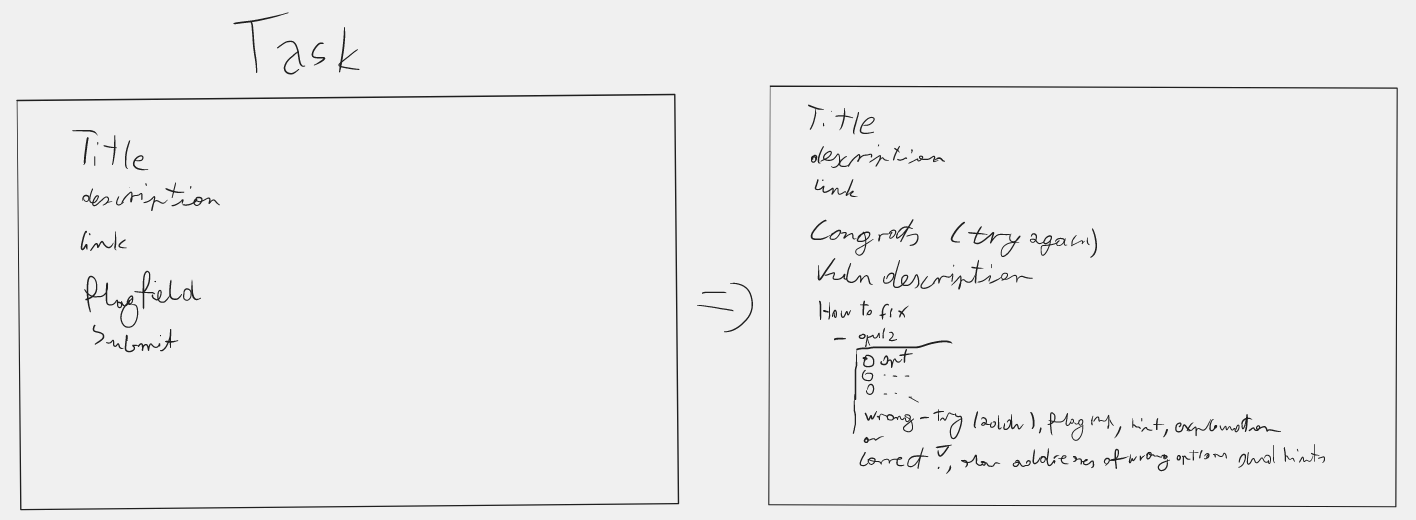
\includegraphics[width=\textwidth]{img/init-ui-sketch.png}
	\caption{Initial task page UI sketch before and after solving the challenge.}
	\label{fig:init-ui-sketch}
\end{figure}

\begin{figure}
	\centering
	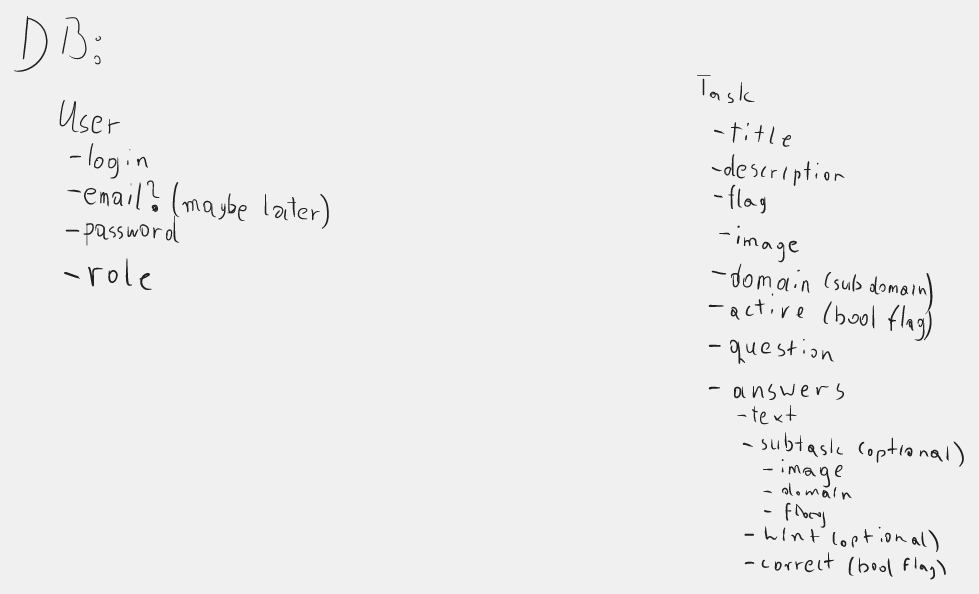
\includegraphics[width=\textwidth]{img/init-db-struct.png}
	\caption{Initial design of documents representing users and tasks.}
	\label{fig:init-db-struct}
\end{figure}

\begin{figure}
	\centering
	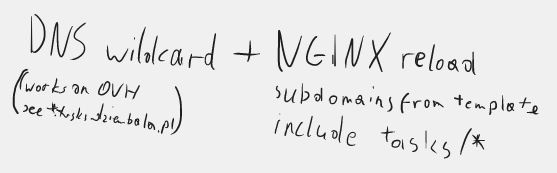
\includegraphics[width=\textwidth]{img/subdomain-idea.png}
	\caption{Subdomain management design idea.}
	\label{fig:subdomain-idea}
\end{figure}

\subsection{Implementation}

The implementation started with setting up a Node.js project with some of the required dependencies and a basic \textit{Hello world} Express server. Additional tools such as ESLint were also set up at the beginning so that they could be used during the development.

The next step was preparing database connection and setting up code for session support. Once the server could handle sessions, related utilities such as message flashing were prepared. Sessions were required to implement authentication, which was done in the next step. The first part of implementing authentication was enabling user account creation, so that it would be possible to test each element as it was developed. With the code responsible for registration ready, logging in could be worked on. In both cases the server logic was prepared first with the UI following right after to test the whole component.

After the authentication was done and there were some simple pages ready, work on styling the interface could begin. This stage of the development was realised at that moment, because there were already pages which could be tested with the styles and could serve as a base for later content.

Before more public pages could be created, an administration panel had to be made in order to insert data for testing. Unlike all other components, this panel required a lot of interactivity and relied on client-side scripting. To facilitate this requirement, the server code exposes REST-like API, which is consumed by scripts running in the browser. The administrator panel started with user management, continued to category management and finished with task creation.\\
Since some of the inputs supported Markdown, a Markdown parser was integrated on both the server and in browser. To allow for syntax highlighting in code blocks, \href{https://highlightjs.org}{highlight.js} was added to the Markdown parser. Syntax highlighting required additional styles, which were available separately in light and dark modes and would not integrate well with Bootstrap's theming. To avoid this problem, a variable-based style sheet with colours from Panda Syntax Light and Dark themes was created with CSS variables set depending on the theme used in Bootstrap.\\
With the last part of the administration panel, task creation, a system for managing challenge containers had to be prepared. During the implementation of this functionality, the initial database schema shown on Fig \ref{fig:init-db-struct} was recognised as suboptimal and had to be changed.

Finally, user-facing category and task pages were prepared. These were template-based and in case of the task page relatively complicated, so the user interface and server code could be implemented in parallel. As a finishing touch a simple home page was added.
